  
\documentclass{beamer}
\usepackage{listings}
\lstset{
%language=C,
frame=single, 
breaklines=true,
columns=fullflexible
}
\usepackage{blkarray}
\usepackage{subcaption}
\usepackage{url}
\usepackage{tikz}
\usepackage{tkz-euclide} % loads  TikZ and tkz-base
%\usetkzobj{all}
\usetikzlibrary{calc,math}
\usepackage{float}
\newcommand\norm[1]{\left\lVert#1\right\rVert}
\renewcommand{\vec}[1]{\mathbf{#1}}
\usepackage[export]{adjustbox}
\usepackage[utf8]{inputenc}
\usepackage{amsmath}
\usepackage{tikz}
\usetikzlibrary{automata, positioning}
\usetheme{Boadilla}
\providecommand{\pr}[1]{\ensuremath{\Pr\left(#1\right)}}
\providecommand{\mbf}{\mathbf}
\providecommand{\pr}[1]{\ensuremath{\Pr\left(#1\right)}}
\providecommand{\qfunc}[1]{\ensuremath{Q\left(#1\right)}}
\providecommand{\fn}[1]{\ensuremath{f\left(#1\right)}}
\providecommand{\e}[1]{\ensuremath{E\left(#1\right)}}
\providecommand{\sbrak}[1]{\ensuremath{{}\left[#1\right]}}
\providecommand{\lsbrak}[1]{\ensuremath{{}\left[#1\right.}}
\providecommand{\rsbrak}[1]{\ensuremath{{}\left.#1\right]}}
\providecommand{\brak}[1]{\ensuremath{\left(#1\right)}}
\providecommand{\lbrak}[1]{\ensuremath{\left(#1\right.}}
\providecommand{\rbrak}[1]{\ensuremath{\left.#1\right)}}
\providecommand{\cbrak}[1]{\ensuremath{\left\{#1\right\}}}
\providecommand{\lcbrak}[1]{\ensuremath{\left\{#1\right.}}
\providecommand{\rcbrak}[1]{\ensuremath{\left.#1\right\}}}
\title{Research Paper Presentation}
\author{Adhvik Murarisetty - AI20BTECH11015}
\date{30th April, 2021}
\begin{document}

\begin{frame}
\titlepage
\end{frame}

\section{}
\begin{frame}{On the Product of Two Correlated Complex
Gaussian Random Variables}
\begin{block}{Abstract}
\begin{enumerate}
    \item We will derive the exact joint PDF of the amplitude and phase of the product of two correlated non-zero mean complex Gaussian random variables with arbitrary variances.
    \item We determine the joint pdf in terms of an infinite summation of modified Bessel functions of the first and second kinds, which generalizes the existing results and observes some special cases. 
    \item We will also study truncation error when a truncated sum is employed.
    \item Finally, we evaluate the derived expressions through numerical experiments.
\end{enumerate}
\end{block}
\end{frame}

\begin{frame}
\begin{block}{Introduction}
Complex Gaussian RVs are used more extensively in signal processing.

We consider the following complex random variable,
\begin{align}
    Z=X Y^*\label{a}
\end{align}
where X and Y are two correlated complex Gaussian RVs
with non-zero means and arbitrary variances. This RV is useful in many applications: 
\begin{enumerate}
    \item In a single channel M-ary phase-shift-keying (MPSK) communication system, the linear combiner output can be characterized by the product of two complex random RVs as \eqref{a}.
    \item In time reversal detection, the aggregate random channel can be modeled by the RV \eqref{a}.
    \item For radar applications, in the case of multipath scattering, for over-the-horizon (OTH) radar for example, the RV is useful to characterize the overall reflection coefficients.
\end{enumerate}
\end{block}
\end{frame}

\begin{frame}
    \begin{block}{NOTATIONS}
    \begin{center}
    \begin{tabular}{ |c|c| } 
    \hline
    SYMBOL & DENOTES \\ 
    \hline
    $\mu,m$ & Mean\\ \hline
    $\sigma$ & Variance\\ \hline
    $\rho$ & Correlation factor\\ \hline
    $E$ & Expectation \\
    \hline
    $(.)^*$ & Conjugate \\ \hline
    $(.)^T $ & Transpose \\\hline
    $(.)^H $ & Conjugate transpose\\\hline
    $j$ & Imaginary unit $\brak{\implies j^2={-1}}$\\\hline
    $ R(.)$ & Real part of a complex number\\\hline
    $ J(.)$ & Imaginary part of a complex number\\\hline
    $I_{\mu}(.)$& Modified Bessel function of first kind with order $\mu$\\\hline
    $K_{\mu}(.)$& Modified Bessel function of second kind with order $\mu$\\
     \hline
    \end{tabular}
    \end{center}
    \end{block}
\end{frame}
\begin{frame}{Some important results}
    \begin{block}{Theorem 1}
    Let $X$ and $Y$ be two bivariate normal random variables,Then there exist independent standard normal random variables $Z_1$ and $Z_2$ such that,
    \begin{align}
        X&=\sigma_X Z_1 +\mu_X\label{3}\\
        Y&=\sigma_Y\brak{\rho Z_1+\sqrt{1-\rho^2}Z_2}+\mu_Y\label{4}
    \end{align}
    \end{block}
    \begin{block}{Proof}
    To prove the theorem, define
    \begin{align}
        Z_1&=\frac{X-\mu_X}{\sigma_Y}\label{1}\\
        Z_2&=-\frac{\rho}{\sqrt{1-\rho^2}}\frac{X-\mu_X}{\sigma_X}+\frac{1}{\sqrt{1-\rho^2}}\frac{Y-\mu_Y}{\sigma_Y}\label{2}
    \end{align}
    Rearranging \eqref{1} will result in \eqref{3} and
    Using \eqref{1} in \eqref{2} will result in \eqref{4}
    \end{block}
\end{frame}
\begin{frame}{Some important results Contd..}
    \begin{block}{Theorem 2}
    Suppose $X\; and\; Y$ are jointly normal random variables with parameters $\mu_X,\;\sigma_X,\;\mu_Y,\;\sigma_Y$ and $\rho$.
    Then, given $X,Y=y$ is normally distributed with,
    \begin{align}
        E[X|Y=y]&=\mu_X+\rho\sigma_X\frac{y-\mu_Y}{\sigma_Y}\label{T1}\\
        \sigma_{{X|Y=y}}&=\brak{1-\rho^2}\sigma_X^2\label{T2}
    \end{align}
    \end{block}
    \begin{block}{Proof}
    Using theorem 1, Let us define
    \begin{align}
        Y&=\sigma_Y Z_1 +\mu_Y\\
        X&=\sigma_X\brak{\rho Z_1+\sqrt{1-\rho^2}Z_2}+\mu_X
    \end{align}
    \end{block}
\end{frame}

\begin{frame}{Some important results Contd..}
    \begin{block}{Proof Contd..}
    Thus given $Y=y$, we have
    \begin{align}
         Z_1&=\frac{y-\mu_Y}{\sigma_Y}
    \end{align}
    and
    \begin{align}
        X&=\sigma_X\brak{\rho \frac{y-\mu_Y}{\sigma_Y}+\sqrt{1-\rho^2}Z_2}+\mu_X\\
        &= \sigma_X\rho \frac{y-\mu_Y}{\sigma_Y}+\sigma_X\sqrt{1-\rho^2}Z_2+\mu_X
    \end{align}
    Since $Z_1\;and\;Z_2$ are independent.  We have shown that given $Y=y,\;X$ is a linear function of $Z_2$, thus it is normal. So,
    \end{block}
\end{frame}
\begin{frame}{Some important results Contd..}
    \begin{block}{Proof Contd..}
    \begin{align}
        E[X|Y=y]&=\sigma_X\rho \frac{y-\mu_Y}{\sigma_Y}+\sigma_X\sqrt{1-\rho^2}E[Z_2]+\mu_X\\
        &=\mu_X+\rho\sigma_X\frac{y-\mu_Y}{\sigma_Y}
    \end{align}
    and
    \begin{align}
        \sigma_{{X|Y=y}}&=\brak{1-\rho^2}\sigma_X^2\sigma_{Z_2}^2\\
        &=\brak{1-\rho^2}\sigma_X^2
    \end{align}
    Since $Z_2$ is a standard normal variable $\implies\;Z_2\sim N(0,1)$ 
    \end{block}
\end{frame}

\begin{frame}{Some important results Contd..}
    \begin{block}{PDF of a complex normal random variable}
    Let $X$ be a complex normal random variable, Then its PDF is 
    \begin{align}
        f_X(x)=\frac{1}{\sigma_X^2\pi}e^{-\frac{|{x-\mu_X}|^2}{\sigma_X^2}}\label{6}
    \end{align}
    \end{block}
     \begin{block}{Important Integrals}
    \begin{align}
        I_{\mu}({u})&=\brak{\frac{u}{2}}^{\mu}\sum\limits_{m=0}^{\infty}\frac{{\frac{u}{2}}^{2m}}{m!(m+\mu)!}\label{I_1}
    \end{align}
    \begin{align}
        \int\limits_0^{\infty} x^{v-1} e^{\brak{-\beta x^ p -\gamma x^{-p}}} dx &= \frac{2}{p}\brak{\frac{\gamma}{\beta}}^{\frac{v}{2p}} K_{\frac{v}{p}}\brak{2\sqrt{\beta\gamma}}\label{I_2}
    \end{align}
    \end{block}
\end{frame}

\begin{frame}{DERIVATION OF JOINT PDF}
    The following theorem provides a general expression for the product of two correlated complex Gaussian random variables.
    
    Let $v=[X,Y]^T\sim CN\brak{m,\Sigma}$ be a $2\times 1$ complex Gaussian vector, where
    \begin{align}
        m=E[v]=[m_x,m_y]^T
    \end{align}
    and
    \begin{align}
        \Sigma&=E\sbrak{(v-m)(v-m)^H}\\&= 
        \begin{bmatrix}
        \sigma_x^2& \rho\sigma_x\sigma_y\\ 
        \rho^*\sigma_x\sigma_y & \sigma_y^2
        \end{bmatrix}
    \end{align}
\end{frame}
\begin{frame}{DERIVATION Contd..}
    \begin{block}{Theorem}
    Let
    \begin{align}
        Z=XY^*=Z_I+jZ_Q=Re^{j\Theta}
    \end{align}
    The joint pdf of $ \brak{R,\Theta}$ is given by
    \begin{multline}
        f_{R,\Theta}\brak{r,\theta}=\frac{2re^{-g}}{c\pi\sigma_y^2}\sum\limits_{n=0}^{\infty}\sum\limits_{p=0}^{\infty}\frac{\beta_1^n\beta_2^p}{n!p!\beta_3^{\frac{n+p}{2}}}\brak{\frac{r^2}{c\alpha}}^\frac{p-n}{2}\\\times K_{p-n}\brak{2r\sqrt{\frac{\alpha}{c}}}I_{n+p}\brak{2\sqrt{\beta_3}}\label{I100}
    \end{multline}
    \end{block}
\end{frame}
\begin{frame}{DERIVATION Contd..}
    Where,
    \begin{align}
        \alpha&=\frac{|b|^2}{c}+\frac{1}{\sigma_y^2}\\
        g&=\frac{|a|^2-2R\cbrak{re^{-j\theta}b}}{c}+\frac{|m_y|^2}{\sigma_y^2}\\
        \beta_1&=\frac{r^2|a|^2}{c^2},\;\;
        \beta_2=|-\frac{b^*a}{c}+\frac{m_y}{\sigma_y^2}|^2 \\
        \beta_3&=2R\cbrak{\frac{re^{-j\theta}a}{c}\brak{-\frac{ba^*}{c}+\frac{m_y^*}{\sigma_y^2}}}
        \end{align}
        in which,
        \begin{align}
            a=m_x-\frac{\rho\sigma_x}{\sigma_y}m_y,b=\frac{\rho\sigma_x}{\sigma_y}\;and\;
            c=\sigma_x^2(1-|\rho|^2)
        \end{align}
        
\end{frame}

\begin{frame}{DERIVATION Contd..}
    The joint pdf for the amplitude R and phase $\Theta$ can be obtained by
    \begin{align}
        f_{R,\Theta}\brak{r,\theta}&=rf_{Z}\brak{r\;cos\theta,r \; sin\theta}\\
        f_{Z}\brak{z_I,z_Q}&=\int\limits_{-\infty}^{\infty}\int\limits_{-\infty}^{\infty}f_{Z|Y}\brak{z_I,z_Q}f_{Y}\brak{y_I,y_Q} \;dy_I\;dy_Q\label{e0}
    \end{align}
    By using \eqref{T1} and \eqref{T2},
    \begin{align}
        X|Y&\sim\;CN\brak{m_X+\rho\sigma_X\frac{Y-m_Y}{\sigma_Y},\brak{1-\rho^2}|\sigma_X|^2}\\
        \implies Z|Y&=XY^*|Y\sim CN\brak{aY^*+b|Y|^2,c|Y|^2}\label{e1}\\
        and\; Y&\sim\;CN\brak{m_y,\sigma_y^2}\label{e2}
    \end{align}
    
\end{frame}

\begin{frame}{DERIVATION Contd..}
    Using \eqref{6},\eqref{e1} and \eqref{e2} in \eqref{e0},
    \begin{align}
         f_{Z}\brak{z_I,z_Q}&=\int\limits_{-\infty}^{\infty}\int\limits_{-\infty}^{\infty}\frac{1}{\pi c|y|^2}e^{-\frac{|{z-\brak{ay^*+b|y|^2}}|^2}{c|y|^2}}\frac{1}{\sigma_Y^2\pi}e^{-\frac{|{y-m_y}|^2}{\sigma_y^2}} \;dy_I\;dy_Q
    \end{align}
    where $y=y_I+jy_Q$ and $z=z_I+jz_Q$
    \begin{multline}
        |{z-\brak{a y^*+b|y|^2}}|^2=|z|^2+|a|^2|y|^2+|b|^2|y|^4-2R\cbrak{z^*a}y_I-2J\cbrak{z^*a}y_Q\\-2R\cbrak{z^*b}|y|^2+2R\cbrak{b^*a}|y|^2y_I+2J\cbrak{b^*a}|y|^2y_Q\label{e3}
    \end{multline}
    \begin{align}
        |{y-\mu_Y}|^2=|y|^2+|m_y|^2-2R\cbrak{m_y}y_I-2J\cbrak{m_y}y_Q\label{e4}
    \end{align}
    Using \eqref{e3} and \eqref{e4} and letting $y_I=t cos\psi$ and $y_Q=t sin\psi$, we will get
\end{frame}
\begin{frame}{DERIVATION Contd..}
     \begin{align}
         f_{Z}\brak{z_I,z_Q}&=\frac{e^{-g}}{c\pi^2\sigma_y^2}\int\limits_{-\infty}^{\infty}\frac{1}{t}e^{-\alpha t^2-\frac{|z|^2}{ct^2}}\int\limits_0^{2\pi}e^{\lambda_1(t,z)cos\psi+\lambda_2(t,z)sin\psi}\;d\psi\;dt\\
         &=\frac{2e^{-g}}{c\pi\sigma_y^2}\int\limits_{-\infty}^{\infty}\frac{1}{t}e^{-\alpha t^2-\frac{|z|^2}{ct^2}}I_0(\lambda(t,z))\;dt\label{e7}
     \end{align}
     where,
     \begin{align}
         \lambda_1(t,z)&=\frac{2R\cbrak{z^*a}}{ct}-\frac{2R\cbrak{b^*a}t}{c}+\frac{2R\cbrak{m_y}t}{\sigma_y^2}\\
         \lambda_2(t,z)&=\frac{2J\cbrak{z^*a}}{ct}-\frac{2J\cbrak{b^*a}t}{c}+\frac{2J\cbrak{m_y}t}{\sigma_y^2}\\
         \lambda(t,z)&=\sqrt{\lambda_1(t,z)^2+\lambda_2(t,z)^2}=2\sqrt{\beta_1 t^{-2}+\beta_2 t^2+ \beta_3}
     \end{align}
\end{frame}
\begin{frame}{DERIVATION Contd..}
    Using \eqref{I_1} to get \eqref{e8} and use it in \eqref{e7},
    \begin{align}
        I_0(\lambda(t,z))&=\sum\limits_{m=0}^{\infty}\frac{({\beta_1 t^{-2}+\beta_2 t^2+ \beta_3})^m}{(m!)^2}\\
        &=\sum\limits_{m=0}^{\infty}\sum\limits_{n=0}^{m}\sum\limits_{p=0}^{n}\frac{(\beta_1 t^{-2})^n(\beta_2 t^{2})^p(\beta_3)^{m-n-p}}{m!n!p!(m-n-p)!}\label{e8}
    \end{align}
    \begin{multline}
       \implies f_{Z}\brak{z_I,z_Q} =\frac{2e^{-g}}{c\pi\sigma_y^2}\sum\limits_{m=0}^{\infty}\sum\limits_{n=0}^{m}\sum\limits_{p=0}^{n}\frac{(\beta_1)^n(\beta_2 )^p(\beta_3)^{m-n-p}}{m!n!p!(m-n-p)!}\\\int\limits_{0}^{\infty}\frac{t^{(2p-2n)}}{t}e^{-\alpha t^2-\frac{|z|^2}{ct^2}}\;dt\label{e9}
    \end{multline}
\end{frame}

\begin{frame}{DERIVATION Contd..}
    Rewiting integral in \eqref{e9} using \eqref{I_2}
    \begin{align}
        \int\limits_{0}^{\infty}\frac{t^{(2p-2n)}}{t}e^{-\alpha t^2-\frac{|z|^2}{ct^2}}\;dt&=\brak{\frac{|z|^2}{c\alpha}}^\frac{p-n}{2}K_{p-n}\brak{2|z|\sqrt{\frac{\alpha}{c}}}
    \end{align}
    \begin{multline}
       \implies f_{Z}\brak{z_I,z_Q} =\frac{2e^{-g}}{c\pi\sigma_y^2}\sum\limits_{m=0}^{\infty}\sum\limits_{n=0}^{m}\sum\limits_{p=0}^{n}\frac{(\beta_1)^n(\beta_2 )^p(\beta_3)^{m-n-p}}{m!n!p!(m-n-p)!}\\\brak{\frac{|z|^2}{c\alpha}}^\frac{p-n}{2}K_{p-n}\brak{2|z|\sqrt{\frac{\alpha}{c}}}
    \end{multline}
    Reordering the summation gives us,
\end{frame}
\begin{frame}{DERIVATION Contd..}
    \begin{multline}
        f_{Z}\brak{z_I,z_Q} =\frac{2e^{-g}}{c\pi\sigma_y^2}\sum\limits_{n=0}^{\infty}\sum\limits_{p=0}^{\infty}\frac{(\beta_1)^n(\beta_2 )^p(\beta_3)^{-n-p}}{n!p!}\brak{\frac{|z|^2}{c\alpha}}^\frac{p-n}{2}\\\times K_{p-n}\brak{2|z|\sqrt{\frac{\alpha}{c}}}\sum\limits_{m=n+p}^{\infty}\frac{\beta_3^m}{m!(m-n-p)!}
    \end{multline}
    \begin{align}
        \sum\limits_{m=n+p}^{\infty}\frac{\beta_3^m}{m!(m-n-p)!}=\brak{\beta_3}^{\frac{n+p}{2}}I_{n+p}\brak{2\sqrt{\beta_3}}\;\; (\therefore using \eqref{I_1} )
    \end{align}
    
     \begin{multline}
       \implies f_{R,\Theta}\brak{r,\theta}=\frac{2re^{-g}}{c\pi\sigma_y^2}\sum\limits_{n=0}^{\infty}\sum\limits_{p=0}^{\infty}\frac{\beta_1^n\beta_2^p}{n!p!\beta_3^{\frac{n+p}{2}}}\brak{\frac{r^2}{c\alpha}}^\frac{p-n}{2} \\K_{p-n}\brak{2r\sqrt{\frac{\alpha}{c}}}I_{n+p}\brak{2\sqrt{\beta_3}}
     \end{multline}
\end{frame}
\begin{frame}{Special Cases}
\begin{block}{Independent RVs}
In this case $\rho=0$, using this in \eqref{I100} gives us
\begin{multline}
    f_{R,\Theta}\brak{r,\theta}=\frac{2re^{-\brak{k_x^2+k_y^2}}}{\pi\sigma_x^2\sigma_y^2}\sum\limits_{n=0}^{\infty}\sum\limits_{p=0}^{\infty}\frac{1}{n!p!}\brak{\frac{k_x}{k_y}}^{n-p} \brak{\frac{|\phi(r,\theta)}{2\sqrt{R\cbrak{\phi(r,\theta)}}}}\\\times K_{p-n}\brak{{\frac{2r}{\sigma_x\sigma_y}}}I_{n+p}\brak{2\sqrt{R\cbrak{\phi(r,\theta)}}}
\end{multline}
    where, $ k_x=\frac{|m_x|}{\sigma_x},k_y=\frac{|m_y|}{\sigma_y}$ and 
    $ \phi(z)=2\frac{R\cbrak{re^{-j\theta m_x m_y^*}}}{\sigma_x^2\sigma_y^2}$.
    
    {This result is agrees with result in \textbf{N. O’Donoughue and J. M. Moura, “On the product of independent
complexGaussians,” IEEE Trans. Signal Process., vol. 60, no. 3, pp. 1050–
1063, Mar. 2012.}}
\end{block}
\end{frame}
\begin{frame}{Special cases contd..}
    \begin{block}{Zero means}
    As $m_x,m_y\to0$ then the terms of \eqref{I100} become,
    \begin{align}
        \lim_{m_x,m_y\to0} g=\frac{-2R\cbrak{re^{-j\theta}b}}{c}=g_0\;and\lim_{m_x,m_y\to0} \beta_i=0,\;i=1,2,3\\
       \implies \lim_{\beta_3\to0}\frac{I_{n+p}\brak{2\sqrt{\beta_3}}}{\beta_3^{\frac{n+p}{2}}}=\lim_{\beta_3\to0}\sum\limits_{m=0}^{\infty}\frac{\beta_3^m}{m!(m+n+p)!}=\frac{1}{(n+p)!}
    \end{align}
    \begin{multline}
        \implies \lim_{m_x,m_y\to0}f_{R,\Theta}\brak{r,\theta}=\lim_{\beta_1,\beta_2,\beta_3\to0,g\to g_0}f_{R,\Theta}\brak{r,\theta}\\
        =\lim_{\beta_1,\beta_2\to0}\frac{2re^{-g_0}}{c\pi\sigma_y^2}\sum\limits_{n=0}^{\infty}\sum\limits_{p=0}^{\infty}\frac{\beta_1^n\beta_2^p}{n!p!}\brak{\frac{r^2}{c\alpha}}^\frac{p-n}{2} K_{p-n}\brak{2r\sqrt{\frac{\alpha}{c}}}\frac{1}{(n+p)!}\label{b1}
    \end{multline}
    \end{block}
\end{frame}
\begin{frame}{Special cases contd..}
    In the \eqref{b1}, the limit of general summation term is non-zero only when n=0,p=0.
    \begin{multline}
        f_{R,\Theta}\brak{r,\theta}=\frac{2re^{-g_0}}{c\pi\sigma_y^2} K_{0}\brak{2r\sqrt{\frac{\alpha}{c}}}\\
        =\frac{2r}{\pi(1-|\rho|^2)\sigma_x^2\sigma_y^2}e^{\frac{2R\cbrak{\rho re^{-j\theta}}}{(1-|\rho|^2)\sigma_x\sigma_y}}K_0\brak{\frac{2r}{(1-|\rho|^2)\sigma_x\sigma_y}}
    \end{multline}
    This result is consistent with result in \textbf{Z. Zheng, L.Wei, J. Hamalainen, and O. Tirkkonen, “A blind time-reversal
detector in the presence of channel correlation,” IEEE Signal Process. Lett.,
vol. 20, no. 5, pp. 459–462, May 2013.}
\end{frame}
\begin{frame}{Truncated joint PDF}
    \begin{block}{Truncated joint PDF}
    Since \eqref{I100} involves a doubly-infinite summation, we define a truncated joint pdf approximation of \eqref{I100} as
    \begin{multline}
        \bar{f}_{R,\Theta}\brak{r,\theta,M}=\frac{2re^{-g}}{c\pi\sigma_y^2}\sum\limits_{n=0}^{M}\sum\limits_{p=0}^{M}\frac{\beta_1^n\beta_2^p}{n!p!\beta_3^{\frac{n+p}{2}}}\brak{\frac{r^2}{c\alpha}}^\frac{p-n}{2} \\\times K_{p-n}\brak{2r\sqrt{\frac{\alpha}{c}}}I_{n+p}\brak{2\sqrt{\beta_3}}\label{I101}
    \end{multline}
    Thus the truncation error is
    \begin{align}
        \epsilon_M= f_{R,\Theta}\brak{r,\theta}-\bar{f}_{R,\Theta}\brak{r,\theta,M}\label{e20}
    \end{align}
    \end{block}
\end{frame}
\begin{frame}{Truncated joint PDF Contd..}
    Substituting \eqref{I100} and \eqref{I101} in \eqref{e20}, using inequalities and approximations, it can be proved that for sufficiently large M, the truncation error \eqref{e20} is bounded by
    \begin{align}
        |\epsilon_m|\le\frac{4re^{-g}}{c\pi\sigma_y^2}\sbrak{\sum\limits_{n=0}^{M+1}\psi_{n,M+1}+\sum\limits_{p=0}^{M+1}\psi_{M+1,p}}=B_M
    \end{align}
    Where,
    \begin{align}
        \psi_{n,p}=\frac{\beta_1^n\beta_2^p}{n!p!|\beta_3|^{\frac{n+p}{2}}}\brak{\frac{r^2}{c\alpha}}^\frac{p-n}{2} K_{p-n}\brak{2r\sqrt{\frac{\alpha}{c}}}I_{n+p}\brak{2\sqrt{\beta_3}}
    \end{align}
    and for any arbitrary $C>1$,
    \begin{align}
        \lim\limits_{M\to\infty}\frac{B_M}{C^{-M}}=0
    \end{align}
    $\implies$ the decay of truncation error is faster than exponential.
\end{frame}
\begin{frame}{Numerical Results}
    Verifying the accuracy of truncated series in \eqref{I101} through numerical results by setting parameters as $$m_x=1, m_y=0.5-j0.5,\sigma_x^2=1,\sigma_y^2=0.8 \;and \;\rho=-\frac{1}{2}e^{j\frac{\pi}{4}}$$
    The below graphs are the cut of truncated PDF along $\theta=0$ and $r=1$ for M=3,4,5,6 and 20.we see that the cuts of the truncated pdf for M = 6 and for M = 20 are almost the same, which implies that for M$>$6, the truncation error can be very small in the tested example.
    
    Other r or $\theta$ cuts of the truncated pdf are also tested and the results are similar.
\end{frame}
\begin{frame}{Numerical Results Contd..}
    \begin{figure}[htp]
    \centering
    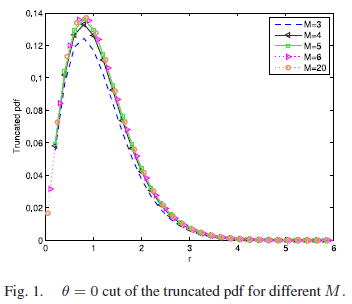
\includegraphics[width=80mm]{030.PNG}
\end{figure}
\end{frame}
\begin{frame}{Numerical Results Contd..}
    \begin{figure}[htp]
    \centering
    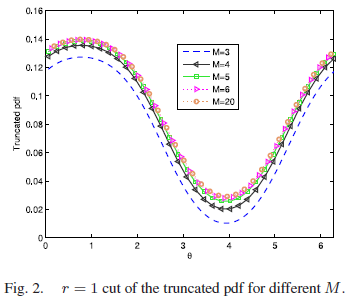
\includegraphics[width=80mm]{031.PNG}
\end{figure}
\end{frame}
\begin{frame}{Numerical Results Contd..}
    Compare the numerical result obtained from Monte- Carlo method with the computation result from \eqref{I101}.
    
    In Fig. 3(a), we plot the numerical result by using $10^7$ independent samples sampled from the RV in \eqref{I100}. In Fig. 3(b), the computation result from \eqref{I101} with M = 20 is plotted.
    
    To evaluate the difference between Fig. 3(a) and Fig. 3(b), define
    \begin{align}
        \epsilon(r,\theta)=|f(r,\theta)- \bar{f}_{R,\Theta}\brak{r,\theta,20}|
    \end{align}
\end{frame}
\begin{frame}{Numerical Results Contd..}
    \begin{figure}[htp]
    \centering
    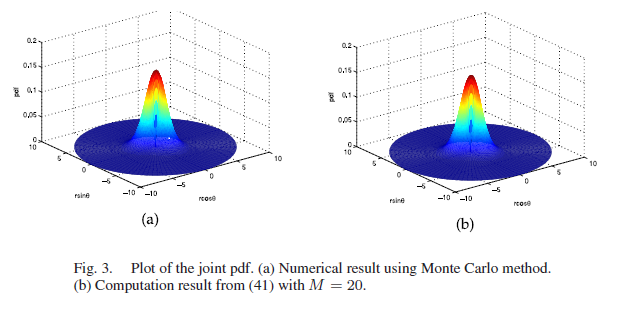
\includegraphics[width=\columnwidth]{0331.PNG}
\end{figure}
\end{frame}
\begin{frame}{Numerical Results Contd..}
    \begin{figure}[htp]
    \centering
    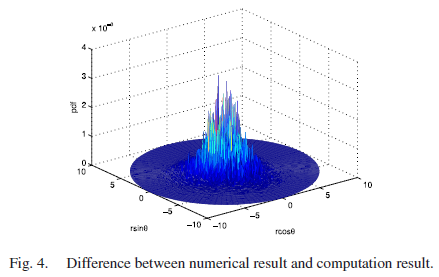
\includegraphics[width=80mm]{034.PNG}
\end{figure}
We see that the peak value of $\epsilon(r,\theta)$ is no larger than $4 \times 10^{-3}$, which is very small compared with the peak values in Fig. 3(a) and Fig. 3(b). This implies that the derived pdf matches numerical result.
\end{frame}
\begin{frame}
   \centering
    \textcolor{blue}{\Huge{\textbf{THANK YOU}}}
\end{frame}
\end{document}
